\chapter{\Dumux Design Patterns}
\label{chap:DesignPatterns}

This chapter tries to give high-level understanding of some of the
fundamental techniques which are used by \Dumux and the motivation
behind these design decisions. It is assumed that the reader already
posseses some basic knowledge in object oriented programming with C++.

First, a quick motivation of C++ template programming is given. Then
follows an introduction to polymorphism and the opportunities for it
opened by the template mechanism. After that, there is a look at some
drawbacks associated with template programming. One of these drawbacks
-- deep nesting of template parameters -- motivates the \Dumux
property system which, in this chapter is outlined from the user
perspective. The chapter concludes with a simple example of how to use
the \Dumux property system.

\section{C++ Template Programming}

One of the main features of modern versions of the C++ language is
robust support for templates. Templates are a mechanism for code
generation build directly into the compiler. To see the motivation of
templates, consider a linked list of \texttt{double} values which
could be implemented like this:
\begin{verbatim}
struct DoubleList {
   DoubleList(const double &val, DoubleList *prevNode = 0)
   { value = val; if (prevNode) prevNode->next = this; };
   double value;
   DoubleList *next;
};
int main() {
   DoubleList *head, *tail;
   head = tail = new DoubleList(1.23);
   tail = new DoubleList(2.34, tail);
   tail = new DoubleList(3.56, tail);
};
\end{verbatim}
But what if a list of strings is also required? The only ``clean'' way
to achive this without templates would be to copy
\texttt{DoubleListNode}, then rename it and change the type of the
\texttt{value} attribute. It should be clear that this is a very
cumbersome and error-prone process, so recent standards of the C++
programming language provide the template mechanism, which is a way
let the compiler do the tedious work. Using templates, a generic
linked list can be implemented like this:
\begin{verbatim}
template <class ValueType>
struct List {
   List(const ValueType &val, List *prevNode = 0)
   { value = val; if (prevNode) prevNode->next = this; };
   ValueType value;
   List *next;
};
int main() {
   typedef List<double> DoubleList;
   DoubleList *head, *tail;
   head = tail = new DoubleList(1.23);
   tail = new DoubleList(2.34, tail);
   tail = new DoubleList(3.56, tail);

   typedef List<const char*> StringList;
   StringList *head2, *tail2;
   head2 = tail2 = new StringList("Hello");
   tail2 = new StringList(", ", tail2);
   tail2 = new StringList("World!", tail2);
};
\end{verbatim}

Compared to code generation approaches using external tools -- which
is the approach chosen for example by the FEniCS~\cite{FENICS-HP}
project -- or heavy use of the C preprocessor -- as done for example
within the UG framework~\cite{UG-HP} -- the template approach has
several advantages:
\begin{description}
\item[Well Programmable:] Programming errors are directly detected by
  the C++ compiler and compiler messages also yield useful information
  since the actual source code is visible to the developer and not
  obfuscated by macros or code generation.
\item[Easily Debugable:] Programs which use the template mechanism can be
  debugged almost as easily as C++ programs which do not use
  templates. This is due to the fact that the debugger always knows
  the ``real'' source file and line number.
\end{description}
For these reasons \Dune and \Dumux extensively use the template
mechanism. Both projects also try to avoid duplicating functionality
provided by the Standard Template Library (STL,~\cite{STL-REF-HP})
which is part of the C++ standard and functionality provided by the
quasi-standard Boost~\cite{BOOST-HP} libraries.

\section{Polymorphism}

In object oriented programming, some functionality often makes sense
for all classes in a hierarchy, but what actually needs to be
\textit{done} can differ for each concrete class. This observation
motivates \textit{polymorphism}. Fundamentally, polymorphism is all
techniques where a method call results in the processor executing code
which is specific to the type of object for which the method is
called\footnote{This is \textit{poly} of polymorphism: There are
  multiple ways to achieve the same goal.}.

In C++, there are two common ways to achieve polymorphism: The
traditional dynamic polymorphism which is not based on template
programming, and static polymorphism which is only made possible by
template programming.

\subsection*{Dynamic Polymorphism}

To utilize \textit{dynamic polymorphism} in C++, the polymorphic
methods are marked with the \texttt{virtual} keyword in the base
class. Internally, the compiler realizes dynamic polymorphism by
storing a pointer to a so-called \texttt{vtable} within each object of
polymorphic classes. The \texttt{vtable} itself stores the entry point
of each method which is declared virtual. If such a method is called
on an object, the compiler generates code which retrieves the method's
address from the object's \texttt{vtable} and then calls it. This
explains why this mechanism is called \textbf{dynamic} polymorphism:
the code which is actually called are dynamically determined at run
time.

\begin{example}
  \label{example:DynPoly}
  A class called \texttt{Car} could feature the methods
  \texttt{gasUsage} which by default corrosponds to the current $CO_2$
  emission goal of the European Union but can be overwritten by the
  classes representing actual cars. Also, a method called
  \texttt{fuelTankSize} makes sense for all cars, but since there is
  no useful default, its \texttt{vtable} entry is set to $0$ in the
  base class which tells the compiler that this method must
  mandatorily be specified by all derived classes. Finally the method
  \texttt{range} may calculate the expected remaining kilometers the
  car can drive given a fill level of the fuel tank. Since the
  \texttt{range} method can retrieve information it needs, it does not
  need to be polymorphic.
\begin{verbatim}
// The base class
class Car
{public:
  virtual double gasUsage() 
  { return 4.5; };
  virtual double fuelTankSize() = 0;
  
  double range(double fuelTankFillLevel) 
  { return 100*fuelTankFillLevel*fuelTankSize()/gasUsage(); }
};
\end{verbatim}

  Actual car models can now derived from the base class:
\begin{verbatim}
// A Mercedes S-class car
class S : public Car
{public:
  virtual double gasUsage() { return 9.0; };
  virtual double fuelTankSize() { return 65.0; };
};

// A VW Lupo
class Lupo : public Car
{public:
  virtual double gasUsage() { return 2.99; };
  virtual double fuelTankSize() { return 30.0; };
};
\end{verbatim}

The \text{range} method called on the base class yields correct result
for any car type:
\begin{verbatim}
void printMaxRange(Car &car)
{ std::cout << "Maximum Range: " << car.range(1.00) << "\n"; }

int main()
{
   Lupo lupo;
   S s;
   std::cout << "VW Lupo:";
   std::cout << "Median range: " << lupo.range(0.50) << "\n";
   printMaxRange(lupo);
   std::cout << "Mercedes S-Class:";
   std::cout << "Median range: " << s.range(0.50) << "\n";
   printMaxRange(s);
}
\end{verbatim}

For both types of cars, \texttt{Lupo} and \texttt{S} the
\texttt{printMaxRange} function works as expected, yielding
$1003.3\;\mathrm{km}$ for the Lupo and $722.2\;\mathrm{km}$ for the
S-Class.
\end{example}

\begin{exc}
What happens if \dots 
\begin{itemize}
\item \dots the \texttt{gasUsage} method is removed from the \texttt{Lupo} class?
\item \dots the \texttt{virtual} qualifier is removed in front of the
  \texttt{gasUsage} method in the base class?
\item \dots the \texttt{fuelTankSize} method is removed from the \texttt{Lupo} class?
\item \dots the \texttt{range} method in the \texttt{S} class is
  overwritten?
\end{itemize}
\end{exc}

\subsection*{Static Polymorphism}

Dynamic polymorphism has a few disadvantages, probably the most
relevant in the context of \Dumux is that the compiler can not see
``inside'' the called methods and thus cannot properly optimize. For
example modern C++ compilers 'inline' short methods, i.e. they copy
the body the method's body to where it is called. This allows to save
a few instructions as well as enables further optimizations which may
depend on specific properties of the function arguments (e.g. constant
value elimination, etc). Inlining and other cross-method optimizations
are next to impossible when using dynamic polymorphism, since these
techniques need to be done by the compiler (i.e. at compile time)
while, for virtual methods, the actual code that gets executed is
determined at run time. To overcome this issue, template programming
can be used to achive polymorphism at compile time. This works by
supplying the type of the derived class as an additional template
parameter to the base class. Whenever the base class needs to call
back the derived class, the \texttt{this} pointer of the base class is
reinterpreted as a derived object and the method is then called. This
scheme gives the C++ compiler complete transparency of the code
executed and thus opens much better optimization oportunities. Since
this mechanism completely happens at compile time, it is called
``static polymorphism'' because the called method cannot be changed
dynamically at runtime.
\begin{example}
  Using static polymorphism, the base class of example \ref{example:DynPoly}
  can be written as
\begin{verbatim}
// The base class. The 'Imp' template parameter is the
// type of the implementation, i.e. the derived class 
template <class Imp>
class Car
{public:
  double gasUsage() 
  { return 4.5; };
  double fuelTankSize() 
  { throw "The derived class needs to implement the fuelTankSize() method"; };
  
  double range(double fuelTankFillLevel) 
  { return 100*fuelTankFillLevel*asImp_().fuelTankSize()/asImp_().gasUsage(); }

protected:
  // reinterpret 'this' as a pointer to an object of type 'Imp'
  Imp &asImp_() { return *static_cast<Imp*>(this); }
};
\end{verbatim}
(Note the \texttt{asImp\_()} calls in the \texttt{range} method.)

The derived classes can now be defined like this
\begin{verbatim}
// A Mercedes S-class car
class S : public Car<S>
{public:
  double gasUsage() { return 9.0; };
  double fuelTankSize() { return 65.0; };
};

// A VW Lupo
class Lupo : public Car<Lupo>
{public:
  double gasUsage() { return 2.99; };
  double fuelTankSize() { return 30.0; };
};
\end{verbatim}
\end{example}

Analogously to example \ref{example:DynPoly}, the two kinds of cars
can be used generically within (template) functions:
\begin{verbatim}
template <class CarType>
void printMaxRange(CarType &car)
{ std::cout << "Maximum Range: " << car.range(1.00) << "\n"; }

int main()
{
   Lupo lupo;
   S s;
   std::cout << "VW Lupo:";
   std::cout << "Median range: " << lupo.range(0.50) << "\n";
   printMaxRange(lupo);
   std::cout << "Mercedes S-Class:";
   std::cout << "Median range: " << s.range(0.50) << "\n";
   printMaxRange(s);
   return 0;
}
\end{verbatim}

\textbf{TODO: Exercise}

\section{Common Template Programming Related Problems}

Although C++ template programming opens a few intriguing
possibilities, it also has a few disadvantages. In this section a few
of those are outlined and some hints how they can be dealt with are
provided.

\subsection*{Blow-Up of Identifiers}

One particular problem with advanced use of templates is that the full
identifier names for types and methods quickly become really long and
unreadable. For example a typical line of an error message generated
using GCC 4.5 in conjunction with \Dune-PDELab looks like
\begin{verbatim}
test_pdelab.cc:171:9: error: no matching function for call to �Dune::\
PDELab::GridOperatorSpace<Dune::PDELab::PowerGridFunctionSpace<Dune::\
PDELab::GridFunctionSpace<Dune::GridView<Dune::DefaultLeafGridViewTraits\
<const Dune::UGGrid<3>, (Dune::PartitionIteratorType)4u> >, Dune::\
PDELab::Q1LocalFiniteElementMap<double, double, 3>, Dune::PDELab::\
NoConstraints, Dumux::PDELab::BoxISTLVectorBackend<Dumux::Properties::\
TTag::LensProblem> >, 2, Dune::PDELab::GridFunctionSpaceBlockwiseMapper>\
, Dune::PDELab::PowerGridFunctionSpace<Dune::PDELab::GridFunctionSpace<\
Dune::GridView<Dune::DefaultLeafGridViewTraits<const Dune::UGGrid<3>, \
(Dune::PartitionIteratorType)4u> >, Dune::PDELab::Q1LocalFiniteElementMap\
<double, double, 3>, Dune::PDELab::NoConstraints, Dumux::PDELab::\
BoxISTLVectorBackend<Dumux::Properties::TTag::LensProblem> >, 2, Dune::\
PDELab::GridFunctionSpaceBlockwiseMapper>, Dumux::PDELab::BoxLocalOperator\
<Dumux::Properties::TTag::LensProblem>, Dune::PDELab::\
ConstraintsTransformation<long unsigned int, double>, Dune::PDELab::\
ConstraintsTransformation<long unsigned int, double>, Dune::PDELab::\
ISTLBCRSMatrixBackend<2, 2>, true>::GridOperatorSpace()�
\end{verbatim}
This seriously complicates diagnostics. Although there is no full
solution for this problem yet, an effective way of dealing with such
kinds of error messages is to ignore the type information and to just
go to the location given at the beginning of the line and also
consider the error text. If nested templates are used and the given
location looks well, the lines above the actual error specify how
exactly the code was instantiated by the compiler (the lines starting
with \texttt{instantiated from}). In this case it is advisable to look
at the innermost location of the code which has been most recently
added.

\subsection*{Proliferation of Template Parameters}

Writing flexible templates often requires a large -- and in some cases
even unknown -- number of template parameters. As an example, the type
of the global operator space from \Dune-PDELab which produced the error
message above is specified like this:
\begin{verbatim}
    enum {numEq = 2};
    enum {dim = 2};
    typedef Dune::UGGrid<2> Grid;
    typedef Grid::LeafGridView GridView;
    typedef Dune::PDELab::Q1LocalFiniteElementMap<double,double,dim> FEM;
    typedef TTAG(LensProblem) TypeTag;
    typedef Dune::PDELab::NoConstraints Constraints;
    typedef Dune::PDELab::GridFunctionSpace<
        GridView, FEM, Constraints, Dumux::PDELab::BoxISTLVectorBackend<TypeTag>
    >
        doubleGridFunctionSpace;
    typedef Dune::PDELab::PowerGridFunctionSpace<
        doubleGridFunctionSpace,
        numEq,
        Dune::PDELab::GridFunctionSpaceBlockwiseMapper
    >
        GridFunctionSpace;
    typedef typename GridFunctionSpace::ConstraintsContainer<double>::Type 
        ConstraintsTrafo;
    typedef Dumux::PDELab::BoxLocalOperator<TypeTag> LocalOperator;
    typedef Dune::PDELab::GridOperatorSpace<
        GridFunctionSpace,
        GridFunctionSpace,
        LocalOperator,
        ConstraintsTrafo,
        ConstraintsTrafo,
        Dune::PDELab::ISTLBCRSMatrixBackend<numEq, numEq>,
        true
    >
        GOS;
    GOS gos; // instantiate grid operator space
\end{verbatim}

Although the code above is not really intuitive, it is not a big
problem if the type in case the grid operator space is only required
at exactly one location. If, on the other hand, it needs to be
consistend over many locations in the source code, something has to be
done in order to keep the code maintainable. The next section outlines
approaches on how to tackle this particular problem.

\section{The \Dumux Property System}
\label{sec:propertysystem}

This section is dedicated to means on how to solve the problem of
template argument proliferation. First, a short look on the more
traditional approach using traits classes is taken, then the design of
the \Dumux property system is explained and finally a short example on
how the system can be used is given.

\subsection*{Traits Classes}

A classic approach to reduce the number of template parameters is to
gather the all arguments in a special class, a so-called traits
class. For example instead of writing
\begin{verbatim}
template <class A, class B, class C, class D>
class MyClass {};
\end{verbatim}
one can use 
\begin{verbatim}
template <class Traits>
class MyClass {};
\end{verbatim}
where the \texttt{Traits} class contains public type definitions for
\texttt{A}, \texttt{B}, \texttt{C} and \texttt{D}, e.g.
\begin{verbatim}
struct MyTraits 
{
  typedef float A;
  typedef double B;
  typedef short C;
  typedef int D;
};
\end{verbatim}

As there is no a free lunch, the traits approach comes with a few
disadvantages of its own:
\begin{enumerate}
\item Trait class hierarchies are problematic. This is due to the fact
  that type defintions must always be defined for the lowest level
  traits class if it is to be used by higher level classes.
\item Traits quickly lead to circular dependencies. This implies that
  types can not be extracted from classes which get the trait class as
  an argument.
\end{enumerate}

To see the point of the first issue, consider the following example:
\begin{verbatim}
struct MyBaseTraits {
  typedef int Scalar;
  typedef std::vector<Scalar> Vector;
};

struct MyDerivedTraits : public MyBaseTraits {
  typedef double Scalar;
};

int main() {
    MyDerivedTraits::Vector v{1.41421, 1.73205, 2};
    for (int i = 0; i < v.size(); ++i)
       std::cout << v[i]*v[i] << std::endl;
}
\end{verbatim}
Contrary to what is wanted, the \texttt{v} variable is a vector of
integers. In this case, static polymorphsism does not come to rescue,
since it would lead to a dependency cycle between
\texttt{MyBaseTraits} and \texttt{MyDerivedTraits}.

The second point is illuminated by the following example, where one
would expect the \texttt{MyTraits::\-VectorType} to be \texttt{std::vector<double>}:
\begin{verbatim}
template <class Traits>
class MyClass {
public:  typedef double ScalarType;
private: typedef typename Traits::VectorType VectorType;
};

struct MyTraits {
    typedef MyClass<MyTraits>::ScalarType ScalarType;
    typedef std::vector<ScalarType> VectorType
};
\end{verbatim}
Although this example seems to be quite pathetic, it is often useful
in reality to specify parameters in such a way.

\subsection*{Features of the \Dumux Property System}

To get around the issues with traits classes, the \Dumux property
system was designed. It can be seen as a traits system which allows
easy type inheritance and any acyclic dependency of types. The scope
at which the property system is executed is completely compile
time. It is based on the following concepts:
\begin{itemize}
\item[Property:] In the context of the \Dumux property system, a
  property is an arbitrary class body which may contain type
  definitions, values and methods. Each property has a so-called
  \textbf{property tag} which can be seen as a label with its name.
\item[Property Inheritance:] Properties can be arranged in
  hierarchies, just like normal classes. Each in the context of the
  \Dumux property system the nodes in the inhertitance hierarchy on
  which the property is defined are called \textbf{type tags}.
\item[Property Nesting:] The definition of a property can depend on
  the value of other properties (as long as there are no cyclic
  dependencies).
\item[Introspection:] The \Dumux property systems supports
  \textbf{diagnostic messages} which can be used to find out how a
  certain property was inherited and where it was defined.
\end{itemize}

\subsection*{\Dumux Property System Reference}

All files where the \Dumux property system is utilized should include
the header file \texttt{dumux/common/propertysystem.hh}, declaration
of new type tags and property tags as well as property definitions
must be done inside the namespace \texttt{Dumux::Properties}.

\subsection*{Defining Type Tags}

New nodes in the type tag hierarchy can be defined using
\begin{verbatim}
NEW_TYPE_TAG(NewTypeTagName, INHERITS_FROM(BaseTagName1, BaseTagName2, ...));
\end{verbatim}
where the \texttt{INHERITS\_FROM} part is optional. To avoid
inconsistencies in the hierarchy, type tags may only be defined
exactly once in the whole program.

\subsubsection*{Declaring Property Tags}

New property tags -- i.e. labels for properties -- are be declared
using
\begin{verbatim}
NEW_PROP_TAG(NewPropTagName);
\end{verbatim}
A property tag can be declared arbitrarily often inside a program, in
fact it is recomended that all properties are declared in each file
where they are used.

\subsubsection*{Defining Properties}

The actual value of a property on a given node of the type tag
hierarchy is defined using 
\begin{verbatim}
SET_PROP(TypeTagName, PropertyTagName)
{
  // arbitrary body of a struct
};
\end{verbatim}
For each a program, a property itself can be declared at most once,
although properties may be overwritten at derived type tags.

Also, the following convenience macros available to define simple
properties:
\begin{verbatim}
SET_TYPE_PROP(TypeTagName, PropertyTagName, type);
SET_BOOL_PROP(TypeTagName, PropertyTagName, booleanValue);
SET_INT_PROP(TypeTagName, PropertyTagName, integerValue);
SET_SCALAR_PROP(TypeTagName, PropertyTagName, floatingPointValue);
\end{verbatim}

\subsubsection*{Unsetting Properties}

\subsubsection*{Converting Tag Names to Tag Types}

For the C++ compiler property and type tags look like ordinary
types. Both can thus be used as template or function arguments,
etc. To convert the name of a property tag or a type tag into the
corrosponding type, the macros \texttt{TTAG(TypeTagName)} and
\texttt{PTAG(PropertyTagName)} ought to be used.

\subsubsection*{Retrieving Property Values}

\begin{verbatim}
GET_PROP(TypeTag, PropertyTag)
\end{verbatim}

Convenience macros:
\begin{verbatim}
GET_PROP_TYPE(TypeTag, PropertyTag)
GET_PROP_VALUE(TypeTag, PropertyTag)
\end{verbatim}

\subsubsection*{Nesting Property definitions}

\subsection*{A Simple Example}

As a concrete example, let us consider some kinds of cars: Compact
cars, sedans, trucks, pickups, military tanks and the Hummer-H1 sports
utility vehicle. Since all these cars share some characteristics it
makes sense to derive the shared properties from the closest matching
car type and only specify the properties which are different. Thus, an
inheritance diagram for the car types above might look like in figure
\ref{fig:car-hierarchy}.

\begin{figure}[t]
  \centering 
  \subfloat[]{
    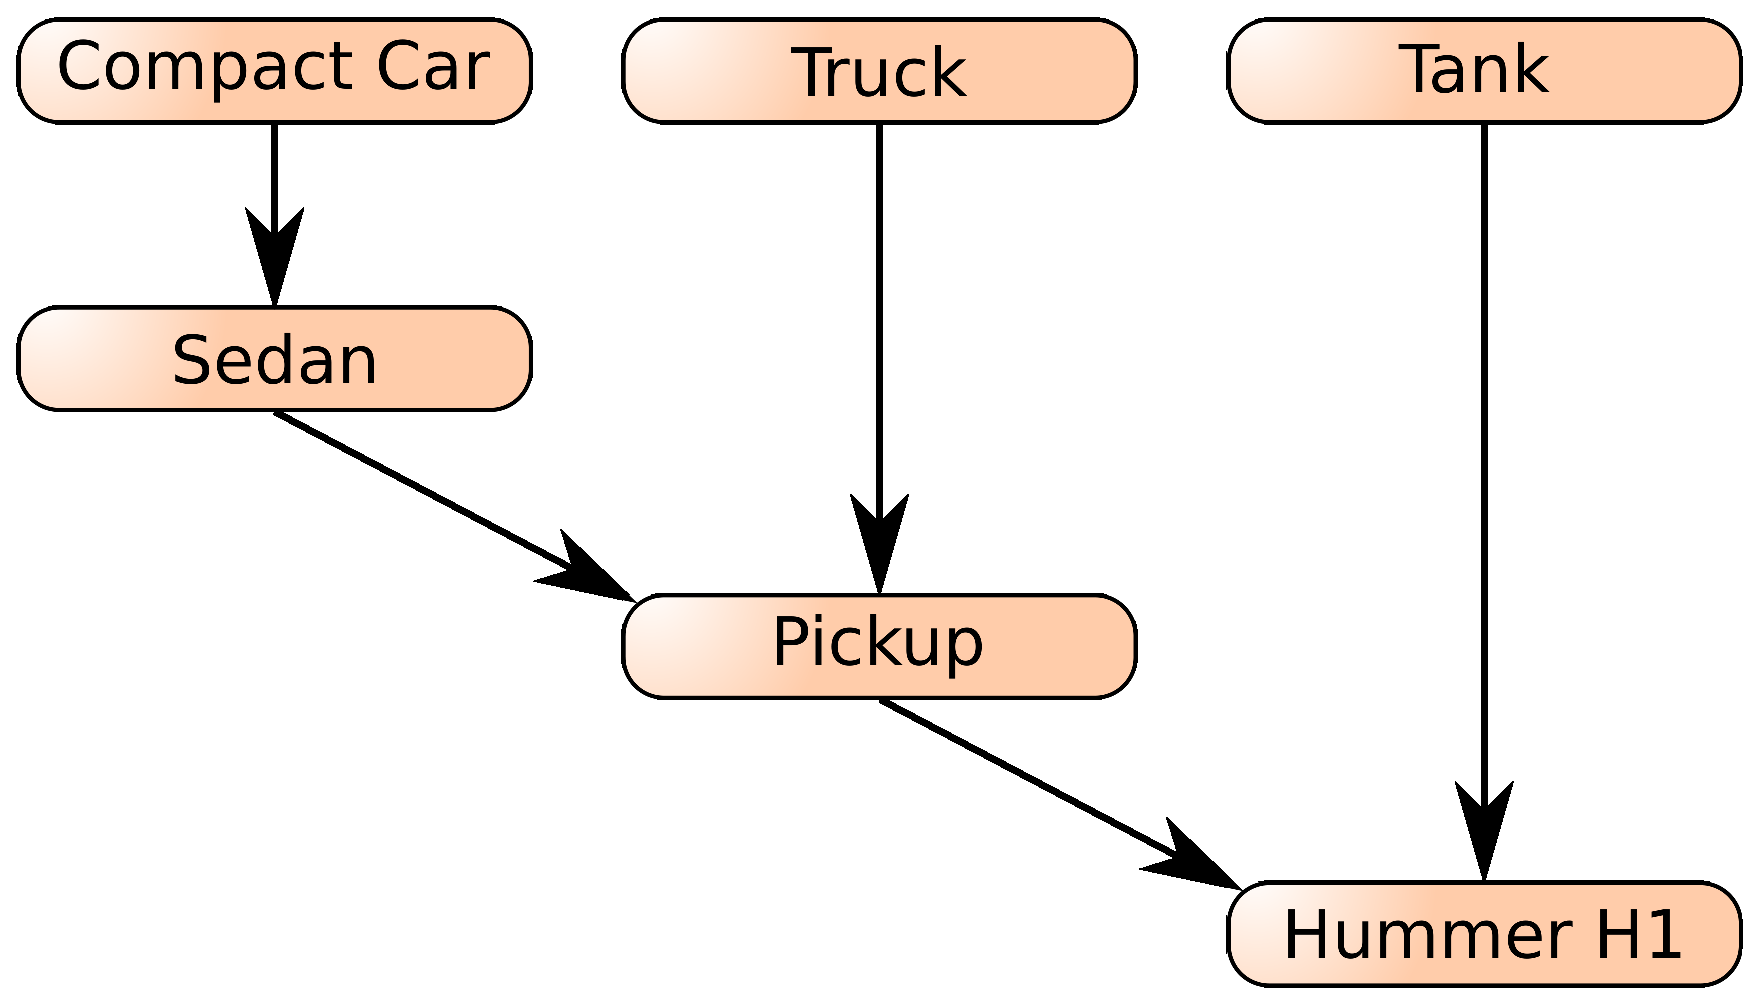
\includegraphics[width=.6\textwidth]{EPS/car-hierarchy.eps}
    \label{fig:car-hierarchy}
  }
  \subfloat[]{
    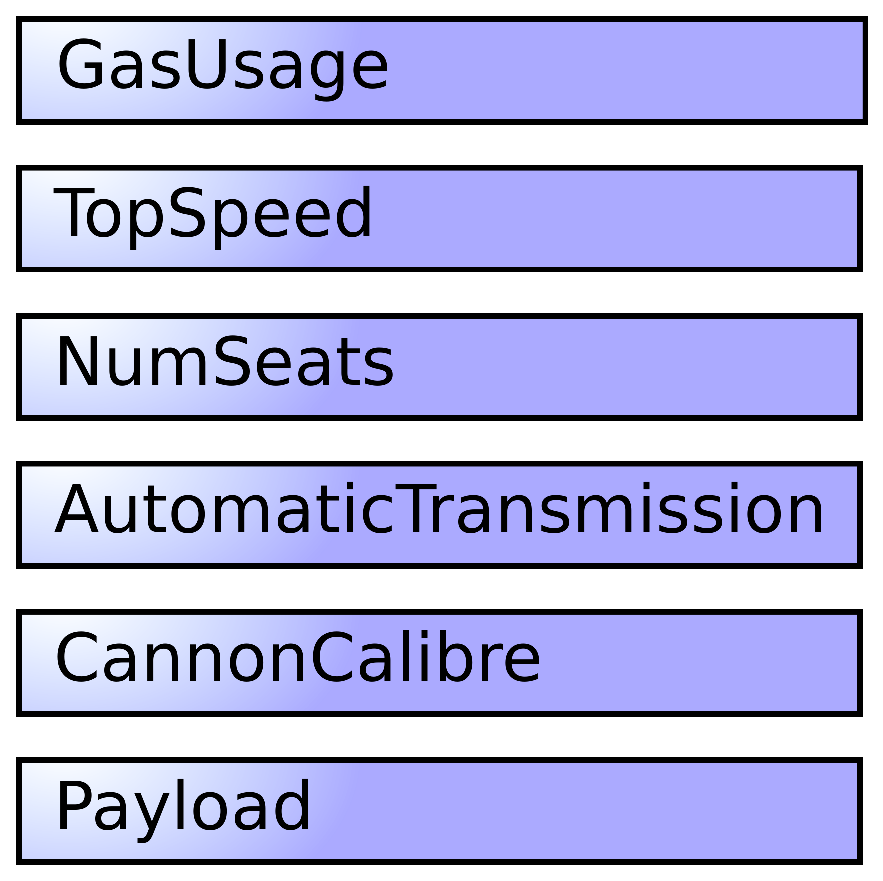
\includegraphics[width=.35\linewidth, keepaspectratio]{EPS/car-propertynames.eps}
    \label{fig:car-propertynames}
  }
  \caption{ \textbf{(a)}~~A possible property inheritance graph for
    various kinds of cars.  The lower nodes inherit from higher ones;
    Inherited properties from nodes on right take precedence over the
    properties defined on the left. ~~\textbf{(b)}~~Property names
    which make sense for at least one of the car types of (a).  }
\end{figure}

Using the \Dumux property system, the inheritance hierarchy can be
defined using
\begin{verbatim}
namespace Dumux {
namespace Properties {
NEW_TYPE_TAG(CompactCar);
NEW_TYPE_TAG(Truck);
NEW_TYPE_TAG(Tank);
NEW_TYPE_TAG(Sedan, INHERITS_FROM(CompactCar));
NEW_TYPE_TAG(Pickup, INHERITS_FROM(Sedan, Truck));
NEW_TYPE_TAG(HummerH1, INHERITS_FROM(Pickup, Tank));
}}
\end{verbatim}

Figure \ref{fig:car-propertynames} lists a few property names which
make sense for at least one of the nodes of figure
\ref{fig:car-hierarchy}. These property names can be declared as
follows:
\begin{verbatim}
namespace Dumux {
namespace Properties {
NEW_PROP_TAG(TopSpeed); // [km/h]
NEW_PROP_TAG(NumSeats); // []
NEW_PROP_TAG(CanonCaliber); // [mm]
NEW_PROP_TAG(GasUsage); // [l/100km]
NEW_PROP_TAG(AutomaticTransmission); // true/false
NEW_PROP_TAG(Payload); // [t]
}}
\end{verbatim}

So far the inheritance hierarchy and the property names are completely
separate. What is missing is setting some values for the property
names on specific nodes of the inheritance hierarchy. Let us assume
the following:
\begin{itemize}
\item For a compact car, the top speed is the gas usage in $l/100km$
  times $30$, the number of seats is $5$ and the gas usage is
  $4\;l/100km$.
\item A truck is by law limited to $100\;km/h$ top speed, the number
  of seats is $2$, it uses $18\;l/100km$ and has a cargo payload of
  $35\;t$.
\item A tank exhibits a top speed of $60\;km/h$, uses $65\;l/100km$
  and features a $120\;mm$ diameter canon 
\item A sedan has a gas usage of $7\;l/100km$, as well as an automatic
  transmission, in every other aspect it is like for a compact car.
\item A pick-up truck has a top speed of $120\;km/h$ and a payload of
  $5\;t$. In every other aspect it is like sedan or a truck but if in
  doubt it is more like a truck.
\item The Hummer-H1 SUV exhibits the same top speed as a pick-up
  truck.  In all other aspects it is similar to a pickup and a tank,
  but if in doubt more like a tank.
\end{itemize}

Using the \Dumux property system, these characteristics can be
expressed using
\begin{verbatim}
namespace Dumux {
namespace Properties {
SET_INT_PROP(CompactCar, TopSpeed, GET_PROP_VALUE(TypeTag, PTAG(GasUsage)) * 30);
SET_INT_PROP(CompactCar, NumSeats, 5);
SET_INT_PROP(CompactCar, GasUsage, 4);

SET_INT_PROP(Truck, TopSpeed, 100);
SET_INT_PROP(Truck, NumSeats, 2);
SET_INT_PROP(Truck, GasUsage, 18);
SET_INT_PROP(Truck, Payload, 35);

SET_INT_PROP(Tank, TopSpeed, 60);
SET_INT_PROP(Tank, GasUsage, 65);
SET_INT_PROP(Tank, CanonCaliber, 120);

SET_INT_PROP(Sedan, GasUsage, 7);
SET_BOOL_PROP(Sedan, AutomaticTransmission, true);

SET_INT_PROP(Pickup, TopSpeed, 120);
SET_INT_PROP(Pickup, Payload, 5);

SET_INT_PROP(HummerH1, TopSpeed, GET_PROP_VALUE(TTAG(Pickup), PTAG(TopSpeed)));
}}
\end{verbatim}

At this point, the Hummer-H1 has a $120\;mm$ canon which it inherited
from its military ancestor. It can be removed by
\begin{verbatim}
namespace Dumux {
namespace Properties {
UNSET_PROP(HummerH1, CanonCaliber);
}}
\end{verbatim}

Now the hierarchy can be queried and some diagnostic messages can be
generated. For example
\begin{verbatim}
int main()
{
    std::cout << "top speed of sedan: " << GET_PROP_VALUE(TTAG(Sedan), PTAG(TopSpeed)) << "\n";
    std::cout << "top speed of truck: " << GET_PROP_VALUE(TTAG(Truck), PTAG(TopSpeed)) << "\n";

    std::cout << PROP_DIAGNOSTIC(TTAG(Sedan), PTAG(TopSpeed));
    std::cout << PROP_DIAGNOSTIC(TTAG(HummerH1), PTAG(CanonCaliber));
}
\end{verbatim}
will yield in the following output:
\begin{verbatim}
top speed of sedan: 210
top speed of truck: 100
Property 'TopSpeed' for type tag 'Sedan'
  inherited from 'CompactCar'
    defined at test_propertysystem.cc:90
Property 'CanonCaliber' for type tag 'HummerH1'
  explicitly unset at test_propertysystem.cc:113
\end{verbatim}


%%% Local Variables: 
%%% mode: latex
%%% TeX-master: "dumux-handbook"
%%% End: 
